\chapter{Towards a Data-Driven Prognostics Approach}

\chapterintrobox{
The aim of this chapter is to present the different prognostic approaches with a detailed taxonomy, the different steps of any prognostic approach will be described and then the emphasis will shift towards data-driven methods.
}

\section{Prognostics of mechanical equipment}
Some complex systems, especially in the oil industry, operate under very severe conditions (offshore, desert, etc.), which can lead to the occurrence of failures and their degradation. Breakdowns and unplanned shutdowns inevitably cause production losses, which can have enormous economic consequences. With these economic constraints, maintenance programs must be developed to minimize the probability of failures, thereby reducing the cost. As discussed in the introduction to this thesis, these programs must be based on the principles of \acrlong{cbm} and \acrlong{phm}.


Prognostics and health management (\acrlong{phm}) has two major aspects \cite{Hess2008}:

\begin{enumerate}
    \item \textbf{Prognostics}: Predictive diagnostics, which includes determining the remaining useful life (service life) of a component or a full system.
    \item \textbf{Health Management}: the ability to make decisions regarding maintenance actions based on diagnostic/prognostic information, available resources and operational demand.
\end{enumerate}

\section{Estimating Remaining Useful Life}
\label{section:rul}
\label{section:rul-estimation}
The main objective of the prognostics is to estimate the remaining useful life (\acrlong{rul}) of the system.
\acrshort{rul} is defined according to the equation \ref{eq:rul}:

\begin{equation}
    RUL = t_f-t_c
    \label{eq:rul}
\end{equation}


Where $t_f$ is the predicted time for the occurrence of the failure and $t_c$ is the current time (the time when the prediction is made).

\section{Physical, Data-Driven and Hybrid Approaches}
\label{section:prognostics-approaches}
Any prognostic approach can be based on physical models, data-driven models or a hybrid combination of the two (Figure \ref{fig:prognostic-approaches-venn}).

\begin{figure}[ht]
    \centering
	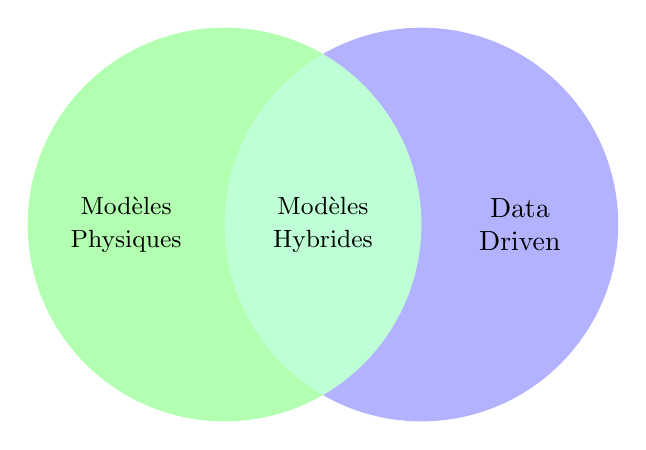
\begin{tikzpicture}
\begin{scope}
[blend group = soft light]
\fill [green!30!white] (0,0) circle (2.5);
\fill [blue!30!white] (2.5,0) circle (2.5);
\end{scope}

\node[text width=2cm, align=center] at (-1.25,0) {\small Modèles Physiques};
\node[text width=1.5cm, align=center] at (3.75,0) { Data Driven};
\node[text width=1.6cm, align=center] at (1.25,0) {\small Modèles Hybrides};
\end{tikzpicture}

    \caption{Classification of prognostics approaches}
    \label{fig:prognostic-approaches-venn}
\end{figure}

These three categories constitute a general classification based on the approach followed, each of which can be subdivided into sub-categories. A detailed taxonomy is presented in Figure \ref{fig:prognostic-approaches-tree}.

\begin{figure}[ht]
	\resizebox{\textwidth}{!}{
\begin{tikzpicture}
	[all/.style={draw, minimum height=2em, fill=white, font=\small}]

	\fill [gray!30!white] (-1.41,-6.3) rectangle (1.41,-9.7) ;
	
	\draw(0,0) node[all] (progApp)                       	{Les Approches du Pronostic};
	\draw node[all, below = 1.6em of progApp] (dataDriv)		{Data-Driven};
	\draw node[all, left = 7em of dataDriv] (physBas)      	{Modèles Physiques};
	\draw node[all, right = 7em of dataDriv] (hybridApp)				{Modèles Hybrides};

	\draw node[all,text width=2cm,align=center,minimum height=3em, below = 1.6em of physBas] (appSpec)		{Application Specific};
	
	\begin{scope}[node distance=1.6em and -3.5em]
		\draw node[all,text width=2cm,align=center,minimum height=3em, below right = of hybridApp] (serApp)		{Approches en Série};
		\draw node[all,text width=2cm,align=center,minimum height=3em, below left = of hybridApp] (parApp)		{Approches Parallèles};
	\end{scope}
	
	\begin{scope}[node distance=1.6em and -2.5em]
		\draw node[all,text width=2cm,align=center,minimum height=3em, below right = of dataDriv] (statMod)		{Modèles Statistiques};
		\draw node[all,text width=2cm,minimum height=3em, align=center, below left = of dataDriv] (ML)		{Machine Learning};
	\end{scope}

	\begin{scope}[node distance=1.6em and 0em]
		\draw node[xshift=1em,all,text width=2.9cm,align=center,minimum height=3em, below left = of ML] (connect) {Méthodes Connectionnistes};
		\draw node[all,text width=2.9cm,align=center,minimum height=3em, below = of connect] (instance) {Apprentissage Contextuel};
		\draw node[ all,text width=2.9cm,align=center,minimum height=3em, below = of instance] (comb)		{Méthodes Combinées};
	\end{scope}

	\begin{scope}[node distance=1.6em and 0em]
		\draw node[xshift=-1em,all,text width=2.9cm,align=center,minimum height=3em, below right = of statMod] (reg)		{Méthodes de Regression};
		\draw node[all,text width=2.9cm,align=center,minimum height=3em, below = of reg] (arma)		{ARMA \& variantes};
		\draw node[all,text width=2.9cm,align=center,minimum height=3em, below = of arma] (propor)		{Modèle à Risque Proportionnel};
	\end{scope}

	\begin{scope}[node distance=1.6em and 0em]
	\path let \p1 = (connect) in node[all,text width=2.3cm,align=center,minimum height=3em] (bayes)	at (0,\y1)	{Méthodes Bayésiennes};
	\draw node[all,text width=2.3cm,align=center,minimum height=3em, below  = of bayes] (hmm)		{Modèles de Markov};
	\draw node[all,text width=2.3cm,align=center,minimum height=3em, below  = of hmm] (sotch)		{Filtrage Stochastique};
	\end{scope}

	\draw[->, >=angle 60] (progApp.south)   -- ++(0,0) -- ++(0,-0.8em) -| (physBas.north);
	\draw[->, >=angle 60] (progApp.south)   -- ++(0,0) -- ++(0,-0.8em) -| (hybridApp.north);
	\draw[->, >=angle 60] (progApp.south)   --  (dataDriv.north);
	
	\draw[->, >=angle 60] (physBas.south)   --  (appSpec.north);
	
	\draw[->, >=angle 60] (hybridApp.south)   -- ++(0,0) -- ++(0,-0.8em) -| (parApp.north);
	\draw[->, >=angle 60] (hybridApp.south)   -- ++(0,0) -- ++(0,-0.8em) -| (serApp.north);
	
	\draw[->, >=angle 60] (dataDriv.south)   -- ++(0,0) -- ++(0,-0.8em) -| (statMod.north);
	\draw[->, >=angle 60] (dataDriv.south)   -- ++(0,0) -- ++(0,-0.8em) -| (ML.north);
	
	\draw[->, >=angle 60] ([xshift=-1em]ML.south)   |- (connect.east);
	\draw[->, >=angle 60] ([xshift=-1em]ML.south)   |- (instance.east);
	\draw[->, >=angle 60] ([xshift=-1em]ML.south)   |- (comb.east);
	
	\draw[->, >=angle 60] ([xshift=1em]statMod.south)   |- (reg.west);
	\draw[->, >=angle 60] ([xshift=1em]statMod.south)   |- (arma.west);
	\draw[->, >=angle 60] ([xshift=1em]statMod.south)   |- (propor.west);

	\draw[->, >=angle 60] (ML.south)   -- ++(0,0) -- ++(0,-0.8em) -| (bayes.north);
	\draw[-] (statMod.south)   -- ++(0,0) -- ++(0,-0.8em) -| (bayes.north);
	\draw[->, >=angle 60] (bayes.south)   -- (hmm.north);
\end{tikzpicture}
}
    \caption{Taxonomy of prognostics approaches \cite{Javed2017}}
    \label{fig:prognostic-approaches-tree}
\end{figure}


\subsection{Physics-based models}
Physics-based models assess the health of the system using an explicit mathematical formulation (white boxes) developed on the basis of a scientific and technical understanding of its behavior. However, the main advantage of these physical models is the use of degradation models to predict long-term behavior \cite{Cubillo2016}. Physical approaches are capable of providing an accurate estimate of the health of the system if the physical model is developed with a complete understanding of the failure mechanisms and efficient estimation of the model parameters. However, for some complex mechanical systems, it is difficult to understand the physics of damage, which limits the application of these approaches \cite{Lei2018}.

\subsection{Data-Driven Models}
\acrlong{dd}  models rely on previously collected data (monitoring data, data on operational parameters, …) to establish a model capable of assessing the health of the system and predicting its behavior and degradation. Contrary to physical models, and as their name indicates, \acrlong{dd} models do not rely on human knowledge but mainly on historical data collected to model the degradation process. Usually, they are considered as black boxes.

\subsection{Statistical Models}
The statistical approach is based on the construction and fitting of a probabilistic model using historical data without depending on any physical or technical principles. 
Si et al. \cite{Si2011} presented a review of statistical approaches. According to this review, many models fall into this category such as regression models (e.g. linear regression), auto-regressive moving average and its variants, stochastic filtering techniques (e.g. Kalman filter, particles filter, …).

\subsection{Machine Learning}
Machine Learning is a field of Artificial Intelligence that has exploded in popularity during recent years and has made breakthroughs in many areas such as computer vision and natural language processing. Machine learning models are black box models that allow even very complex mappings from input to output to be discovered. Many types of algorithms fall into this category such as connectionist methods (e.g. artificial neural networks), context learning (e.g. support-vector machines). Different approaches can be combined together to create mixed models that may perform better than a single model.

\subsection{Hybrid Models}
Hybrid models are a combination of a physical model and an \acrlong{dd} model. There are two types of hybrid models depending on how the two types of models are combined. The \acrlong{dd} model can be integrated into a physical model in a series configuration (Figure \ref{fig:hybrid-approach-series}) where it is used to adjust the parameters of the physical model which is then used to make predictions.

\begin{figure}[H]
    \centering
    \begin{tikzpicture}
 	\node[draw, rectangle] (ph) {Physics based approach};
 	\node[draw, rectangle, below = 3em of ph] (dd) {Data-driven approach};
 	
 	\draw[->, >=angle 60] (dd.north) -- node[right] {\scriptsize  Parameter tuning} (ph.south);
 	\draw[->, >=angle 60] (ph.east) -- node[above] {\scriptsize Prediction} ([xshift=4.5em]ph.east);
 	\draw[->, >=angle 60] (-4.5,0) -- node[above] {\scriptsize Input} (ph.west);
	\draw[->, >=angle 60] (-3,0) |-  (dd.west);
\end{tikzpicture}
    \caption{Series hybrid configuration (Figure adapted from \cite{Mangili2013})}
    \label{fig:hybrid-approach-series}
\end{figure}

The two types of models can be combined in a parallel configuration (Figure \ref{fig:hybrid-approach-parallel}) where the two models make separate predictions that can be combined to obtain the final estimate.

\begin{figure}[H]
    \centering
    \begin{tikzpicture}
    \node[draw, rectangle] (ph) {Physics based approach};
    \node[draw, circle, below = 1em of ph] (u) {U};
    \node[draw, rectangle, below = 1em of u] (dd) {Data-driven approach};

    \draw[->, >=angle 60] (u.east)      --      node[above] {\scriptsize Prediction} ([xshift=4.5em]u.east);
    \draw[->, >=angle 60] (ph.south)    --      (u.north);
    \draw[->, >=angle 60] (dd.north)    --      (u.south);
    \draw[->, >=angle 60] (-4.5,0)      --      node[above] {\scriptsize Input} (ph.west);
    \draw[->, >=angle 60] (-3,0)        |-      (dd.west);
    %the following lign is just to make the figure center precisely and align with the previous one
    \draw[->, draw=none] (ph.east) -- ([xshift=4.5em]ph.east);
\end{tikzpicture}
    \caption{Parallel hybrid configuration (Figure adapted from \cite{Mangili2013})}
    \label{fig:hybrid-approach-parallel}
\end{figure}


\section{Why a Data-Driven Approach?}
As mentioned previously, understanding the degradation process for very complex systems is extremely difficult, which is why the development of physical models is very problematic for these systems.

The last 20 years have seen great progress in the development of new detection techniques, prognostics/diagnostics methods and in the application of computer-aided analysis methods. 

It is interesting to note that at the 2002 workshop on condition-based maintenance organized by the Advanced Technology Program of the United States National Institute of Standards and Technology (NIST), the following obstacles to the widespread application of CBMs were identified:
\begin{itemize}% [label=$\bullet$]
    \item The impossibility of accurately and reliably predicting the remaining service life of a machine.
    \item The inability to continuously monitor a machine.
    \item The Inability of maintenance systems to learn and identify impending failures and recommend action.
\end{itemize} 

These barriers can be redefined as deficiencies in prognosis, detection and reasoning. These and other limitations in the current implementation of condition-based maintenance techniques have, of course, been recognized by others and have led to the development of programs (e.g. in the military field) to overcome them \cite{Hess2008}.

Today, sensors in industry have become inexpensive and ubiquitous, computing power has increased exponentially which has allowed the development of more advanced algorithms and computing tools: the artificial intelligence revolution and machine learning. The industry generates huge amounts of data in many areas, the majority of which is untapped. Exploiting this data using the latest technological advances can increase profits, drastically reduce costs and prove to be a huge economic advantage.

\section{Conclusion}
Adoption of data-driven prognostics models can be helpful especially when behavior of degradation process is ambiguous and developing physics-based models to quantify the health state of complex systems is complicated and their results become unreliable. Recent developments in sensoring techniques, increase in available computation power (i.e. faster and cheaper processing units) and also abundance of—unexploited—monitoring data has provided the needed framework for adopting these data-driven models which are easier to develop, deploy and automate than their physics-based counterparts.
